~
\newpage
\section{Designing Climate Policy}

\subsection{A Case for Economic Analysis in Climate Policy Design}

There is a tremendous need for scientific research into emissions reducing technology. In the International Energy Agency's plan to achieve net zero emissions by 2050, currently available technologies can only sustain abatement through 2030. By 2050 only half of the technology needed to reduce emissions is currently on the market. The agency estimates that governments worldwide will need to immediately invest over \$90 billion into key areas of research and development like electrification and carbon capture technologies---areas that currently receive only about \$25 billion in research funding \citep{ieareport}. 

Given that the physical sciences have alerted the world to the destructive potential of climate change and occupy a central role in creating abatement technologies, it seems reasonable to question why the global response to climate change should incorporate economic analysis. There is an apparent tension between mitigating climate change damages and protecting the economy. While I address the nature of this tension more in the following section, the cost-benefit analysis that underlies much of the discipline feels inappropriate when it comes to environmental issues. Why should we care about money when the fate of the planet is at risk?

\begin{figure}
	\centering
	\caption{Climate Cynicism}
	
\includegraphics[scale=0.2]{figures/chapter2_figures/dino.jpg}\\
	%\footnotesize This is a rough draft so I'm allowed to have this
\end{figure}

There are a few necessary clarifications to make regarding this question. First, economic tradeoffs exist whether or not we acknowledge them, and these tradeoffs are not always simple. Consider an impoverished community with a coal-burning power plant. The plant emits sulfur dioxide into the air, which can lead to respiratory issues. But if the plant is to reduce its emissions and continue operating, the cost of electricity will likely rise and hurt the already poverty stricken community. Workers at the plant may lose their careers. Though troublesome, there is a tradeoff here between public health and poverty alleviation. In the context of climate change, \cite{nordhaus2019climate} notes in his Nobel lecture:
\begin{quote}
	``If, for example, attaining the 1.5°C goal would require deep reductions in living standards in poor nations, then the policy would be the equivalent of burning down the village to save it. If attaining the low-temperature path turns out to be easy, then of course we should aim for it."
\end{quote}
Economists generally try to quantify these competing interests and place them in terms of a common unit, the dollar.\footnote{Expressing costs and benefits in terms of dollars is often  convenient though not necessary. For instance, \cite{carleton2020valuing} express climate change adaptation costs not in dollars, but in terms of ``statistical lives."} The question of climate mitigation costs and benefits may seem irrelevant or even unethical to some observers, but the economics discipline has the methodological tools to inform potential skeptics.

Second, money is the primary concern of firms engaged in emissions producing activities. The economics discipline largely concerns itself with the incentives of both firms and consumers---incentives that if designed well, can lead to substantial emissions reductions. Money undoubtedly plays a role in determining whether or not people drive electric cars, manufacturers install smokestack scrubbers, and electric power producers build fossil fuel generators. Even if we concede that bringing the world down to net zero emissions is invaluable, public policy that does not systematically consider how firms and consumers will react risks failure. In a global crisis at the scale of climate change, the potential costs of this risk are substantial. 

Lastly, despite what some political pundits might propagate, the economic consensus is remarkably clear: climate change is a major threat that warrants significant action. In a 2021 survey of climate economists, 74\% said that climate change necessitates ``immediate and drastic action." Less than 3\% answered that either ``more research is needed before action is taken" or that climate change ``is not a serious problem" \citep{howard2021gauging}.\footnote{Another 24\% said that ``some action should be taken now" on climate change.} Although it may seem trivial to some, economists largely agree that the benefits of bold climate policy outweigh the costs. The economic perspective adds further credibility to the case for climate policy, particularly when much of the criticism lodged at climate action focuses on its cost. 

In summary, economics provides a quantitative and systematic approach to making potentially difficult decisions related to our relationship with the Earth's atmosphere and our environment. This is approach is not without its flaws, but it is one of many important perspectives. Not only does economic analysis allow us to consider the tradeoffs of specific policy proposals, but it provides theory and empirical techniques essential to identifying how firms and individuals will respond to policy. Climate economists predominantly agree that climate change urgently deserves bold public policy, a view that aligns with climate scientists and researchers at large. While physical scientific research can develop the technologies that permit emissions reductions, research in economics and other social sciences will be integral in the successful adoption of these technologies and related behavioral changes.


\subsection{An Economic Motivation for Climate Policy}

The general approach advocated by policymakers begins by making the production of electric power less carbon intensive. This involves the familiar steps of switching from coal power plants, to wind and solar farms. This is called \emph{decarbonization} of the electric power grid. Simultaneously, policymakers need to transition energy-using activities to rely on electric power, rather than other forms of energy. Electric vehicles are the most popular push for electrification. Some greenhouse gas emissions are likely inevitable, so bringing the world to net zero emissions requires that those emissions are offset through increased carbon sequestration, the removal and storage of CO$_2$ emissions from the atmosphere. The tree is a simple carbon sequestration device, but difficult to use at the necessary scale. Carbon sequestration technology requires significant public investment, but unlike decarbonization and electrification, this does not need to involve many economic actors.

\begin{figure}
\caption{Market for an Emissions Intensive Good}
\centering
\begin{tikzpicture}[scale=0.6]
	\draw[very thick, EAPblue, domain=0:12] plot (\x, {.8*\x + .4}) node[right]{MPC};
	\draw[very thick, EAPyellow, domain=0:12] plot(\x, {.4*\x}) node[right]{MD};
	\draw[very thick, EAPgreen, domain=0:8] plot(\x, {1.2* \x + .4}) node[right]{MSC};
	\draw[very thick, EAPred, domain=0:12] plot (\x, {-.5*\x + 9}) node[right]{D = MB};
	\draw[thick, dashed] (6.615, 0) node[below]{$Q^*$} -- (6.615, 5.692) -- (0, 5.692) node[left]{$p^*$};
	\draw[thick, dashed] (5.059, 0) node[below]{$Q^S$} -- (5.059, 6.471) -- (0, 6.471) node[left]{$p^S$};
	\draw[very thick, <->] (0,10) node[left]{$p$} -- (0,0) -- (13,0) node[below]{$Q$};
\end{tikzpicture}
\end{figure}

To the economist, the problem lies in the universal impact of greenhouse gas emissions. Greenhouse gas emissions, and almost any type of pollution, are a fundamental example of an externality, where an economic activity has consequences on agents outside of the activity. For one driver, the impact of one more gallon of gasoline used on the climate is entirely negligible, and the cost she incurs for that next gallon of gasoline is just the price at the gas station. Unfortunately, she is not the only person who incurs the costs of the induced climate change---so do the other seven billion people on the planet.\footnote{There are additional externalities here related to how this activity will affect future generations. The extraction of the oil for gasoline production prevents future generations from extracting and using that same unit of oil. Future generations will also feel the climate effect caused by present emissions. In both cases, the value of these damages are highly dependent on the discount rate assumed.} This cumulative effect may still be small, but is no longer negligible. However, she does not face the burden of climate change damages incurred by all other people caused by her driving. These costs are external to the driver when she chooses how much gas to put in her car or what car to buy in the first place. 

Related to these externalities, the shared nature of the atmosphere and climate create excludability complications. Modern economic theory classifies goods according to two criteria: rivalry and excludability.\footnote{ \cite{ostrom2010beyond} reviews the historical development of the four goods commonly used today. The seminal paper \cite{samuelson1954pure} moved the discipline away from just private goods and described a public good, introducing the excludability criterion. Although \cite{hardin1968tragedy} popularized the concept of rivalrous goods, club goods were first formally introduced in \cite{buchanan1965economic} and open-access goods were first formally introduced in V. Ostrom and E. Ostrom (\citeyear{ostrom1977public}).} If we accept the double dichotomies of a good either being excludable or non-excludable and rival or non-rival, then these criteria lead to four types of economic goods: private goods, public goods, open-access goods, and club goods. These goods and the good matrix are shown in Figure \ref{goods}.

A clean atmosphere is a public good. All people can benefit from a healthy atmosphere with greenhouse gases at a level that supports climate stability, and one person's benefit does not infringe on another's. By the same virtue, greenhouse gas emissions are a public bad. No individual can exclude herself from climate change, and one person's high climate change damages do not prevent someone else from also experiencing high damages. The difficulty in public goods lies in finding out how to pay for them. Economists often use the classic prisoners' dilemma game to model a public good contribution game. All agents have a strictly dominant strategy to not contribute towards the public good, provided that they would prefer to not contribute to the public good and not receive it than finance the public good individually. A coal-burning power plant wants to prevent climate change damages, but preventing these damages will require sweeping action from around the world. It could not successfully mitigate climate change damages by itself, and even if it could, the costs involved would far exceed its benefits. If other actors choose to take aggressive action on climate change, then making serious abatement efforts costs the coal plant but provides no benefit. In either case, the plant is better off doing nothing. The universal, non-excludable nature of the benefits of climate change mitigation fails to create the proper incentives for individual actors to take action.\footnote{The rivalry of goods tends to be less important than their excludability in environmental contexts. \cite{hardin1968tragedy} famously considered the example of an English pasture to show that agents will overexploit non-excludable but rival goods, leading to the collapse of the natural system, provided the agents have no institutions that can enforce cooperation. For this reason, the excludability is the primary concern in the environmental and climate settings.}

\begin{figure}
\caption{A Taxonomy of Goods}
\label{goods}
\centering
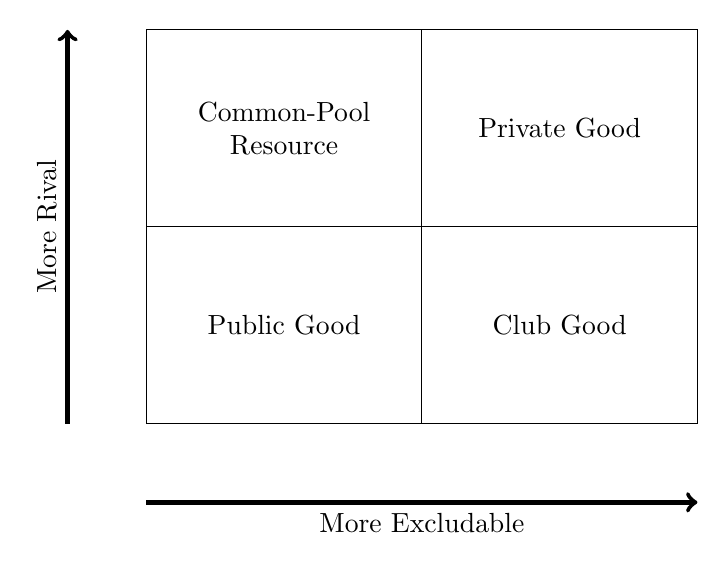
\begin{tikzpicture}[scale = 0.5]
	\draw (0,0) rectangle (7,5) node[pos=.5] {Public Good};
	\draw (7,5) rectangle (14,10) node[pos=.5] {Private Good};
	\draw (0,5) rectangle (7,10) node[pos=.5, text width = 2.5cm, align=center] {Common-Pool Resource};
	\draw (7,0) rectangle (14,5) node[pos=.5] {Club Good};
	\draw[ultra thick, ->] (0,-2) -- (14, -2) node[pos =.5, below]{More Excludable};
	\draw[ultra thick, ->] (-2, 0) -- (-2, 10) node[pos =.5, above, rotate=90]{More Rival};
\end{tikzpicture}
\end{figure}

Absent any additional incentive, individual agents will fail to implement the necessary changes. In some rare instances, economic actors can in theory internalize the externality through bargaining, a result known as the Coase theorem \citep{coase1960problem}. This implies that occasionally, private agents can resolve externalities without government intervention. The Coase theorem has found only limited use in environmental applications. For the Coase theorem to hold even theoretically, there must be enforceable property rights and transaction costs must be negligible. These transaction costs are often substantial, especially when dealing with many different actors and assessing compliance is difficult. Because climate change involves quite literally every person on the planet (and many more people not yet born), it suffices to say that serious efforts at curbing climate change cannot be made without government involvement. Further, Coasean bargaining may have potentially troubling distributional consequences. However, bargaining will likely play a pivotal role in any successful international climate agreements. In these contexts, we can consider how bargaining may be able to address climate change without an international government. Even this will require national governments to implement strong climate policy.

Putting these pieces together, individual firms and consumers will emit far too many greenhouse gas emissions as the costs they face do not reflect the greater societal costs of their actions. These same firms and consumers will fail to produce a cleaner atmosphere, a necessary public good, because they cannot exclude others from enjoying the benefit of a clean atmosphere. Without this ability to exclude, those willing to produce a cleaner atmosphere will not do so because individuals do not have an incentive to buy a cleaner atmosphere. Without buyers, there can be no market for a clean atmosphere. The market failure that leads to climate change is less of a market failure and much more of a market omission. The omission of the market for a clean atmosphere creates ragged, incomplete edges in adjacent emissions intensive markets. Finally, the scope of the problem is so large that resolution of climate change through private actors is not only impractical, but too costly to be increasing welfare.


\subsection{The Structure \& Scope of Environmental Policy}

In Garrett Hardin's classic work ``The Tragedy of the Commons,"  he proposes two approaches to managing open-access resources: private ownership and state ownership. The key in both cases is the centralization of control over the commons---centrality which allows other actors to be excluded from  the commons. Decades later, Elinor Ostrom critiqued this dichotomy in her landmark book \textit{Governing the Commons}, in which she documents many cases from around the world where non-government institutions have successfully sustained resources including grazing land, forests, and groundwater aquifers. In each of these cases, individuals and firms organized themselves in ``collective action" to protect natural resources. 

Could similar approaches like those Ostrom studies succeed in creating climate action? It is highly unlikely. Both Hardin and Ostrom focus on open-access resources, where a healthy atmosphere is firmly a public good (alternatively, greenhouse gas emissions are a public bad). Much of their analysis is based on the rivalry of the resources and consequently does not translate well for reducing emissions. More importantly, some of the key features that allow these self-governance approaches to succeed are not met in the context of climate change. The systems Ostrom studies are primarily local and rely on mutual-monitoring and enforcement. Given the global nature of climate change and the invisibility of greenhouse gas emissions, it would be a tremendous leap to say that climate action is achievable through self-governance and collective action alone. It is not surprising that current climate policy in the US predominantly resembles the dichotomy espoused by Hardin. This same dichotomy appears in US environmental policy as well.

The inevitability of the incentive-induced failure of private management of the climate crisis forces public policy. Still, there is a wide variety of tools available to policymakers for addressing environmental and climate issues. 
%Figure \ref{policies} highlights the major types of environmental policies using classifications adapted from \cite{keohane2016markets}. 
Analogous to Hardin's dichotomy, environmental policy typically falls into one of two categories: \emph{market-based policy} and \emph{command-and-control policy}. Command-and-control policies create changes by enforcing directives, while market-based policies make use of primarily financial incentives.

Command-and-control policies are what we would typically think of as environmental regulation. Here, government creates specific prescriptions to firms and possibly consumers. For this reason, command-and-control policy is also often called \emph{prescriptive policy}. Prohibition policies prevent actors from taking certain actions, like purchasing a piece of public land or disposing of a hazardous chemical. These typically appear in the management of public lands, like National Parks, Wildlife Refuges, and Forests. Often alongside prohibition is permission, where government may for instance lease National Forests to the logging industry or grant rights to a firm to drill for oil on state-owned land. In a loose sense, we might also classify any policy enforcement as a part of this category. Regulators may prohibit certain activities with prescribed punishments for violators. 

Another approach to regulating and protecting the environment is through standard setting. Standards are generally either \emph{technology standards} or \emph{performance standards}. Technology standards require firms to use specific technologies. Many coal-burning power plants must install smokestack scrubbers to prevent damaging chemicals from entering the lower atmosphere. Alternatively, performance standards do not specify specific technologies, but set bounds on the rate or total magnitude of an environmental impact. This could involve setting an emissions cap on an individual firm or car fuel economy standards, which indirectly govern the rate of carbon dioxide emissions per mile. The discipline lacks clear definitions for some of these classifications, and occasionally performance standards form a category between market-based and command-and-control policies. Technology standards provide the characteristic inflexibility of a command-and-control policy, but performance standards can provide somewhat more flexibility. 

Information tools can use a combination of both command-and-control and market-based policies. For instance, a mandatory eco-labeling program might require firms to display the carbon footprint of a good they sell. This a specific reporting requirement without a direct financial incentive attached to the policy. Still, consumers, seeing this information might change what and how many products they purchase. This creates secondary financial incentives for firms, similar to a market-based policy. Sometimes these programs are not mandatory, and firms  voluntary participate in labeling due to some financial incentive. Other times, there is no financial incentive for information disclosure, but regulators require disclosure regardless. This is the case in program's like the EPA's Greenhouse Gas Emissions Reporting Program. This program requires facilities that have potential high emissions to collect data and report on their greenhouse gas emissions.

Generally, market-based policies operate instead not by imposing specific rules, but instead by creating those essential but missing markets. Policymakers primarily do this through the two components of any market: price and quantity.  Price instruments are the traditional Pigouvian solution. When there is a market failure due to some externalitiy, we can internalize the externality by taxing or subsidizing a good so individual incentives will align with social incentive. Carbon taxes are a clear example of this strategy. There are costs of carbon dioxide emissions that do not appear in the prices of goods and activities that rely on these emissions. A carbon tax creates a financial incentive for firms and consumers to reduce their emissions. It also it flexible---no individual has to change her behavior, but continued emissions will come at a cost.  Analogous programs subsidize energy-efficient goods, providing a financial incentive to adopt durables that will use less energy and reduce emissions. 

Alternatively, policymakers might also use quantity-based instruments to create financial incentives. The typical example here is a cap-and-trade program, where policymakers require certain actors to own emissions permits or emissions allowances for every ton of their greenhouse gas emissions. Policymakers create a fixed quantity of these permits and can sell these to regulated firms. If firms were only allowed to keep these emissions allowances, then this would be equivalent to a performance standard. The key piece of the differentiation is the tradeable nature of these allowances. Under a cap-and-trade program, firms can buy and sell these emissions allowances from each other. This creates a market for allowances, which puts a price on emissions. Just like a carbon tax, the price of an emissions allowance creates a financial incentive for emissions abatement. Other programs outside of the reduction of greenhouse gas emissions make use of quantity-based instruments. For instance, Wetland Mitigation Banking in the US fixes a quantity of land for wetland conservation. Firms and farmers that wish to develop on existing wetland must offset this development by building or conserving a tract of wetland equivalent to the wetland they displace through development. 

% \begin{landscape}
% \begin{figure}
% \centering
% \caption{Taxonomy of Major Environmental Policies \label{policies}}
% \begin{tikzpicture}[grow = down, scale = 1, semithick]
% 	\footnotesize
% 	\tikzstyle{level 1}=[level distance=20mm,sibling distance=9cm]
%     \tikzstyle{level 2}=[level distance=5cm,sibling distance=4.5cm]
%     \tikzstyle{level 3}=[level distance=5cm,sibling distance=4.5cm]
        
%     \tikzstyle{s1}=[rectangle, rounded corners, text width=4cm, draw, inner sep = 5, fill = white, semithick,fill opacity = 0,text opacity = 1, minimum height = 4cm]
%     \tikzstyle{s1-mod}=[rectangle, rounded corners, text width=4cm, draw, inner sep = 5, fill = white, semithick,fill opacity = 0,text opacity = 0, draw opacity=0, minimum height = 4cm]
%     \tikzstyle{s2}=[rectangle, rounded corners, text width=6cm, draw, inner sep = 5, fill = white, semithick,fill opacity = 0,text opacity = 1]
%     \tikzstyle{s3}=[rectangle, rounded corners, text width=6cm, draw, inner sep = 5, fill = white, semithick,fill opacity = 0,text opacity = 1]
%     \tikzstyle{s4}=[rectangle, rounded corners, text width=4cm, draw, inner sep = 5, fill = white, semithick,fill opacity = 0,text opacity = 1]
    
	
% 	\node[s3, text centered]{Major Environmental Policy Options}
% 		child{node[s2, text centered]{Market-Based Policies}
% 			child{node[s1]{Price Tools
% 				\begin{itemize}
% 					\item Carbon taxes
% 					\item Border carbon adjustments
% 					\item Energy-efficiency subsidies
% 				\end{itemize}
% 			}
% 				edge from parent node[]{}}
% 			child{node[s1]{Quantity Tools
% 				\begin{itemize}
% 					\item Cap-and-trade
% 					\item Individual fishing quotas
% 					\item Wetland mitigation banking
% 				\end{itemize}							
% 			}
% 				edge from parent node[]{}}
% 			child{node[s1-mod]{I}
% 				edge from parent node[]{}}
% 			edge from parent node[]{}}
% 		child{node[s2, text centered]{Command-and-Control Policies}
% 			child{node[s1]{Information Tools
% 				\begin{itemize}
% 					\item Eco-labelling programs
% 					\item Green building certification
% 					\item Emissions reporting
% 				\end{itemize}
% 			}
% 				edge from parent node{}}
% 			child{node[s4]{Standard Setting}
% 					child{node[s1]{Performance-Based
% 							\begin{itemize}
% 								\item Minimum vehicle fuel efficiency standards
% 								\item Minimum ambient air quality standards
% 							\end{itemize}
% 						}
% 						edge from parent node[]{}}
% 					child{node[s1]{Technology-Based
% 							\begin{itemize}
% 								\item Smokestack scrubber requirements
% 								\item Sewage discarge equipment requirements
% 							\end{itemize}
% 						}
% 						edge from parent node[]{}}
% 				edge from parent node[]{}}
% 			child{node[s1]{Prohibition and Permission
% 				\begin{itemize}
% 					\item Endangered species protection
% 					\item Conservation land
% 					\item Drilling rights on public land
% 				\end{itemize}							
% 			}
% 				edge from parent node[]{}}
% 			edge from parent node[]{}};
% \end{tikzpicture}
% \vspace{.25cm}
% \begin{minipage}{0.8\textwidth}
% 	\footnotesize
% 	Classifications and examples developed from \cite{keohane2016markets}. 
% \end{minipage}
% \end{figure}
% \end{landscape}

So what policies are most effective? Economists tend to favor market-based over command-and-control approaches in many contexts for two primary reasons. First, market-based approaches are in a theoretical sense, cost-effective. That is, well-designed price and quantity tools can achieve environmental targets while minimizing the burden of regulation on firms and consumers. This seems somewhat ironic. Many environmental issues are fundamental examples of market failure, yet here the implication is that these same issues are best resolved inside of a market. \cite{keohane2016markets} perhaps say it best ``the problem is not that markets are so pervasive but that they are not pervasive \emph{enough}---that is, they are incomplete." Are economists naive to suspect that the same free-market principles that cause environmental issues can actually resolve them? The section that follows expands on this question by providing an example of why carbon taxes and cap-and-trade programs can be reasonably cost-minimizing, and some justification of why command-and-control policies are not. Later sections will address this empirically and show that market-based tools can be effective in resolving environmental and climate issues.

Second, market-based programs create incentives for firms to invest in research and development of new technologies with positive environmental impacts. Under a technology standard, firms have no interest in creating new technologies. Doing so would only impose additional and unnecessary costs on themselves. Additionally, if firms encountered technologies with the potential to reduce their environmental impact, they would have an incentive to hide it from public and particularly from regulators. Under a market-based approach, firms have a strong incentive to innovate new technologies. With a carbon tax, major innovations in abatement technology would allow firms to save on emissions costs, giving them a strong competitive advantage. If firms could anticipate future increases in the price of emissions, they might even make this investment even if the current emissions price was relatively low.
 
Despite the apparent merits of market-based approaches to environmental policy, price and quantity instruments are no panacea. One significant concern in many areas of environmental policy is enforcement. Natural resources are often incredibly large and it is difficult to monitor individual behaviors that relate to these resources. The earlier discussion on the cost-minimizing nature of these market-based approaches excludes any consideration of enforcement costs. What happens if we incorporate these costs into our analysis?

For instance, say we wanted to reduce bycatch on commercial fishing vessels. Bycatch is when fishers unintentionally catch sealife like dolphins or sea turtles instead of the fish they intended to catch. There are ways fisher can mitigate bycatch, like using specific kinds of nets that allow some species to escape.
Consider a market-based strategy to reduce bycatch, like taxing fishers for the non-targeted sea life that they catch and kill. If fishers followed this rule, the tax would be enough for many of them to adopt the technologies that would reduce bycatch. This would minimize the total costs incurred by fishers. Fishers who face high costs from reducing bycatch will barely reduce their bycatch as they would rather pay the tax. Fishers who face low costs from reducing bycatch will greatly reduce their bycatch as they would rather adopt new technologies than pay a tax. Of course, this assumes that there is perfect compliance and enforcement is costless. What kind of costs would be involved in enforcing a tax like this? Monitoring and taxing the bycatch of every commercial fisher in an area would be tremendously difficult and expensive. We do not have the technology to monitor every animal caught in every commercial fishing nets. Even there was a monitoring official on every large commercial vessel, there would be strong incentives for collusion. 

In situations where enforcement is incredibly costly, it may be more cost-effective to take a command-and-control approach that prescribes uniform policies across actors. In this example, it would much less expensive to require that commercial fishers use bycatch-reducing nets. Policymakers could incorporate this into existing procedures for commercial fishing licensing and even prevent the production and sale of more harmful nets. This policy would not be cost-minimizing for the fishers, but if the difference in enforcement costs was large enough, it may be more cost-minimizing to society as a whole. A technology standard, a command-and-control approach, seems more appropriate in this case.


\subsection{Environmental Markets: Carbon Taxes \& Cap-and-Trade}

To illustrate the theory behind these polices, consider the example of carbon taxes and cap-and-trade programs. The market missing in climate change is a market for emissions abatement. Figure \ref{abatement1} displays this market. The supply of emissions abatement is equivalent to the marginal abatement costs (MAC). Towards the left of the MAC curve are the low hanging fruit of abatement options.\footnote{Some empirical estimates of this curve suggest that this far portion of the MAC may actually be negative. That is, initial emissions abatement is achievable at a negative cost, as firms and individuals can often save money through energy-efficiency improvements. This is related to the energy-efficiency gap \citep[see][]{allcott2012there, gerarden2017assessing}.} As more abatement occurs, the technologies involved in abatement become more costly, and many of these require new research investments into technologies that are not yet available. 

Although there are private costs involved in emissions abatement, there are also social gains. These gains are equivalent to avoided climate change damages. Marginal damages increase with the quantity of emissions; the more emissions are already in the atmosphere, the greater the impact of an extra ton of CO$_2$. For this reason, the marginal benefits of abatement are decreasing. The first ton of CO$_2$ abated is responsible for the largest reduction in climate change damages, and any subsequent abatement is less effective at reducing damages. Abatement is a public good though, so despite the social benefits, no private agents are willing to pay for abatement. 

Market-based policies attempt to resolve this issue by using government to act as a ``demander" of abatement. It is impractical for policymakers to set a full demand curve for abatement, so instead policymakers can set clearer demand curves that will still bring the market to its true equilibrium. Namely, a policymaker can set a horizontal demand curve for abatement at $p^*$ or a vertical demand curve for abatement at $A^*$. These two options are identical in simple models of abatement as both lead to the socially optimal level of abatement. 

\begin{figure}
\caption{Creating a Market for a Public Good (or Bad)}
\centering
\subcaptionbox{The Market for Abatement \label{abatement1}}{
\begin{tikzpicture}[scale=0.45]
	\draw[very thick, <->] (0,10) node[left]{$p$} -- (0,0) -- (13,0) node[below]{$Q$}; 	
	\draw[very thick, EAPred, domain=0:12] plot(\x, {.6*\x + 1}) node[right]{\footnotesize S = MAC};
	\draw[very thick, EAPblue, domain=0:12] plot(\x, {-.4*\x + 9}) node[right]{\footnotesize D = MB}; 
	\draw[very thick, lightgray] (8,0) node[below, black]{$A^*$} -- (8,10);
	\draw[very thick, lightgray] (0,5.8) node[left, black]{$p^*$} -- (13,5.8);
	\draw[very thick] (11, 0) node[below]{$A_\text{Max}$} -- (11, 10);  
	\node[below] at (6.5, -3) {Abatement ($A$)};
	\draw (9.5, -2) node{$\underbrace{~~~~~~~~~~}_{E^*}$};
\end{tikzpicture}
}
\hspace{.01cm}
\subcaptionbox{The Market for Emissions \label{emissions1}}{
\begin{tikzpicture}[scale=0.45]
	\draw[very thick, <->] (0,10) node[left]{$p$} -- (0,0) -- (13,0);	
	\draw[very thick, EAPred, domain=0:12] plot(\x, {7.6 - .6*\x}) node[above right]{\footnotesize D = MB};
	\draw[very thick, EAPblue, domain=0:12] plot(\x, {4.6 + .4*\x}) node[right]{\footnotesize S = MSC};
	\draw[very thick] (11, 0) node[below]{$E_\text{Current}$} -- (11, 10);
	\draw[very thick, lightgray] (3,0) node[below, black]{$E^*$} -- (3,10);
	\draw[very thick, lightgray] (0,5.8) node[left, black]{$p^*$} -- (13,5.8);	
	\node[below] at (6.5, -3) {CO$_2$ Emissions ($E$)};
	\draw (7, -2) node{$\underbrace{~~~~~~~~~~~~~~~~~~~~~~~~~~~}_{A^*}$};
\end{tikzpicture}
}
\end{figure}

The previous example framed market-based instruments from the perspective of creating a market for emissions abatement. 
%This approach highlights how government intervention can work to establish a market for a public good. Additionally, it makes use of the marginal abatement cost curve which is often relatively easy to estimate in practice. 
Although this framing is important and one that is often more convenient, the interpretation and public policy implications can seem counterintuitive. With government on the demand side, this would imply a policy where government pays polluters to abate, either promising a fixed rebate on each ton of emissions abated or by purchasing abatement until it reaches $A^*$. In this system, polluters would earn more revenue by through abatement. Major climate policy proposals do not include such massive payoffs to polluters, and rightly so; in the long run these economic profits would attract more firms to enter high-polluting industries and diminish the efficacy of policy. There may also be additional social costs if government reduces other expenditures or raises taxes in order to finance these payouts. 

The familiar policies focus on the inverse of the abatement market, the market for emissions. This market appears in Figure \ref{emissions1}. In this market, the government does not intervene to demand a public good, but to establish rights for and supply a public bad. The polluters derive their demand for emissions from their MAC curves---it represents the most polluters will be willing to pay for the right to send CO$_2$ emissions into the atmosphere rather than abate. The supply curve in this market is the marginal damage of emissions. This framing comes with a clearer interpretation. Here, policymakers impose a carbon tax---a charge of $p^*$ on each ton of CO$_2$ emissions. In equilibrium, this tax will lead to total emissions $E^*$. A cap-and-trade program program instead sets a vertical supply curve of emissions allowances, permits that give polluters the right to emit one ton of CO$_2$, at $E^*$. A key feature of these allowances is that they are tradeable between polluters. Although it is not necessary for government to sell or auction off emissions allowances, if government did, their equilibrium price would be $p^*$. 

The market for abatement and the market for emissions correspond. The difference between the maximum level of abatement and the equilibrium level of abatement is the equilibrium emissions, and the difference between the current level of emissions and the equilibrium level of emissions is the equilibrium abatement. The market price for emissions is the same as the market price for abatement. Framing market-based policy through the market for emissions has a more convenient interpretation relative to standard policy. However, because the prices and quantities are identical in both markets, economists often choose to frame market-based polices through the market for abatement rather than the market for emissions. This approach can be clearer when considering the cost-minimizing nature of market-based instruments.

\begin{figure}
\caption{Distribution of Allowances \label{dist_allowance}}
\centering
\begin{tikzpicture}[scale=0.7]
	\draw (0,0) rectangle (10,8.33);
	\draw (0,0) node[below]{0} -- (10,0) node[below]{100} -- (10,8.33) node[above]{0} -- (0,8.33) node[above]{100} -- (0,0);
	\draw[very thick, ->] (10, 9.33) -- (0, 9.33) node[pos=.5, above]{Polluter 2's Abatement (tons)};
	\draw[very thick, ->] (0, -1) -- (10, -1) node[pos=.5, below]{Polluter 1's Abatement (tons)};
	\draw[very thick, EAPred, domain=0:9.603] plot(\x, {.09*\x^2});
	\draw[very thick, EAPblue, domain=3.988:10] plot(\x, {.1*(12-\x)^2 + 1.91}); 
	\draw[thick, dashed] (0,4.41) node[left]{\$50} -- (7,4.41);
	\draw[thick, dashed] (7,8.33) node[above]{30} -- (7,0) node[below]{70};
	\node[rotate=90, above] at (-1, 4.155) {Price (\$)};
	\node[EAPred] at (9, 5.5) {MAC$_1$};
	\node[EAPblue] at (9, 1.5) {MAC$_2$};
	\draw[lightgray, thick] (5,0) node[below, black]{50} -- (5,8.33) node[above, black]{50};
\end{tikzpicture}
\end{figure}

It turns out that in our simple theoretical model of a cap-and-trade program with tradeable allowances, the original distribution of allowances is irrelevant to whether or not the policy achieves the emissions reduction cost-effectively. Suppose that there are just two polluters in our system, Polluter 1 and Polluter 2, each of whom currently has 100 tons in emissions. The assumed benevolent policymaker wants to cut emissions in half by setting a cap of 100 tons of emissions. Polluter 1 and 2 have marginal cost of abatement curves depicted in Figure \ref{dist_allowance}. Consider two alternative scenarios: (1) the policymaker sells allowances to the polluters, and (2) the policymaker gifts 50 (tradeable) allowances to each polluter. 

If the policymaker sells allowances to the polluters, then both polluters will purchase allowances up until the price of an allowance equals the cost of an additional ton of abatement. That is, each polluter will purchase the quantity of emissions allowances where the price of an allowance is equal to its marginal abatement cost. The demand for abatement is perfectly inelastic, so the equilibrium price will be where the sum of the quantities of abatement supplied by the polluters is 100 tons. Graphically, the total marginal abatement cost curve for the two polluters together is a horizontal summation of each individual marginal abatement cost curve. Figure \ref{dist_allowance} shows that at a price of \$50, the sum of the Polluter 1 and 2's abatement is 100 tons, the desired level of abatement. Total abatement costs are equal to the area under each abatement curve from 0 to its level of abatement. Figure \ref{dist_allowance} shows that this allocation minimizes this area. 

Suppose instead each polluter begins with 50 allowances. If both have 50 allowances, Polluter 2 would have a far higher marginal cost of abatement than Polluter 1. Knowing this, Polluter 1 might sell some of its allowances to Polluter 2. Polluter 1 will sell its allowances as long as the price it receives is at least as high as its marginal abatement cost. Polluter 2 will buy allowances as long as the price it pays is weakly less than its marginal abatement cost. These dynamics bring the market to equilibrium where Polluter 1 sells 20 of its allowances to Polluter 2 at a price of \$50 per allowance. As before, this allocation of emissions and abatement minimizes total abatement costs. This shows that even if the two allowances are distributed uniformly and freely to polluters with heterogeneous marginal abatement costs, we still reach the cost-minimizing allocation of emissions abatement. 

The major difference is not in the total costs, but in the distribution of these costs. If the policymaker uses an auction to allocate the allowances, then Polluter 1 will pay less (total) than Polluter 2, but both will bear the cost of purchasing emissions allowances and abatement costs; the cost of these allowances becomes government revenue. If the policymaker uniformly distributes the allowances between polluters, then Polluter 1 will collect additional revenues from selling 20 allowances, Polluter 2 will bear additional costs from buying another 20 allowances, and both bear their abatement costs. 

Although the optimal distribution of allowances is highly normative, conventional economic thought suggests that the auction method may have a slight welfare advantage over the gifting of allowances. Selling the emissions rights is considered \emph{non-distortionary}, as it corrects an existing market failure. If government used these additional revenue to reduce distortionary taxes, then this could lead to welfare gains in other pieces of the economy. We return to the question of how policymakers might choose to allocate allowances when we consider the European Union's Emission Trading System and the approach its policymakers had used up until recently to address emissions leakage risk.


\subsection{Incomplete Carbon Markets: Competition, Leakage, and Border Carbon Adjustments}

\begin{quote}
	``You know these pest control companies. They call themselves exterminators, but they can't really do it. The best they can do is get the bugs to go to somebody else's house. They just relocate them, you know what I mean? They're bug realtors is what they are."
	--- Jerry Seinfeld (Seinfeld, Season 6, Episode 19, ``The Doodle")
\end{quote}
	
Previously, we have looked at the ability of carbon pricing schemes (either an emissions tax or an emissions trading program) to reduce greenhouse gas emissions within a closed economy. Although this is a standard example of Pigouvian approaches to tackling externalities, the story is more complex when we instead consider an open economy. 

When an individual country/state/city takes up a carbon pricing scheme, we call this a \emph{unilateral} carbon pricing scheme, meaning that this jurisdiction adopts the policy without coordinated carbon pricing schemes across all or most all other jurisdictions. This is the current state of carbon pricing schemes. According to the \cite{wbank}, 21\% of all anthropogenic greenhouse gas emissions faced an emissions price in 2021. Even if Country A has a price on its carbon, it will not be able to put a price on the emissions from Country B, even though Country B's emissions are just as damaging to Country A as its own emissions. That is not to say that unilateral carbon pricing schemes are not worth it, but to acknowledge that there is something missing. This is an example of an \emph{incomplete regulation}: a situation where not all relevant actors in the market face regulation. In the case of greenhouse gas emissions, everyone is a relevant actor, meaning that without a global carbon pricing scheme, any unilateral carbon pricing scheme will always be incomplete. In this section, we begin to explore the implications of the incompleteness of unilateral emissions pricing and analyze possible solutions.

%The fundamental issue that leads to emissions leakage is that unilateral carbon pricing schemes are incomplete forms of regulation. We say that a regulation is incomplete if not all relevant actors in the market face regulation. In a closed economy, a unilateral carbon tax would not induce emissions leakage; all the actors in the market are subject to the carbon tax. This is not the case for the open economies of the real world, prompting the need for additional policies to complement the initial regulation.

\textbf{The Big Picture of Climate Policy \& Competition}

A frequent claim of those opposing aggressive climate policy is that it will make the country less economically competitive relative to other countries.\footnote{Do I dare include something from MTG on this: ``[Supporters of the Green New Deal] want to shut down our economy, they want to end  our energy independence and surrender America, putting us on our knees to China--dependent on China, yes, just to drive a car or a truck. That is not in some distant time in the future. That is pretty soon, especially in less than 10 years\ldots They want to transform America into a Third World country, and that is exactly what these policies will do" \citep{marjorie_greene}.} Here, I will use the term ``competitive" in the sense that foreign firms will gain a greater global market share, usually as a result of lower costs. Understandably, the effect of climate and environmental policy on economic activity (both domestic and foreign) is of considerable interest to not just economists, but policymakers and the general public.

The contemporary literature on the relationship between economic standard of living and environmental decay begins with Simon Kuznets, and his work related not to the environment, but inequality. \cite{kuznets1955economic} laid out a empirical relationship between economic development and inequality. Kuznets findings suggest that income inequality rises as countries move from low-income to middle-income, and income inequality falls as countries move from middle-income to high-income. Diagrammatically, this creates an inverted U-shaped path called the Kuznets Curve with GDP per capita on the horizontal axis and measures of inequality (usually the income ratio between the top quintile and bottom quintile of earners) on the vertical axis. Realizing that economic development and environmental degradation follow a similar relationship, \cite{NBERw3914} were the first to formulate the \emph{Environmental} Kuznets Curve (EKC) in an analysis of NAFTA. While the model was not the primary focus of the original paper, it later led to its own published paper, \cite{grossman1995economic} and is now a standard in environmental economics. 

Figure \ref{EKC} displays the Environmental Kuznets Curve. The EKC hypothesizes that low-income economies will have relatively high environmental quality, as these economies may be more agrarian or pastoral. Countries often move from low-income to middle-income through industrialization, and as countries industrialize, their environmental degradation increases. Eventually though, economic development requires countries to move away from manufacturing and into higher human capital industries. When this happens, sectors dependent on high human capital (e.g., finance, engineering, education) tend to be less harsh on the environment. Past the turning point, economic development will decrease environmental degradation. 

\begin{figure}
\centering
\begin{minipage}{0.48 \textwidth}
\caption{The EKC \label{EKC}}
\begin{tikzpicture}[scale = 0.6]
\draw[thick, <->] (0,10) -- (0,0) -- (10,0);
\draw[thick, EAPblue]  [domain = 1:9] plot (\x, {8.5 - .5*(\x - 5)^2});
\node [below right] at (7,0) {GDP/Capita};
\node[rotate=90, above] at (0,7) {Environmental Degradation};
\draw[dashed] (5,0) -- (5,9.5) node[right]{\footnotesize Turning Point};
\end{tikzpicture}
\end{minipage}
\begin{minipage}{0.48\textwidth}
\centering 
\caption{Application of the  EKC}
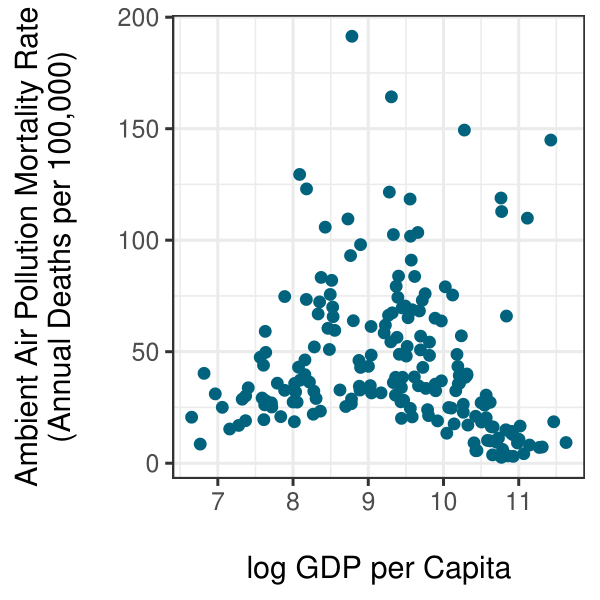
\includegraphics[width=0.9\textwidth]{figures/chapter2_figures/ekc.png}
\end{minipage}
Data from \cite{owidoutdoorairpollution} 
%https://ourworldindata.org/outdoor-air-pollution#outdoor-air-pollution-tends-to-rise-with-industrialization-before-falling
\end{figure}

Despite its quick adoption in the discipline and its continued use, the EKC has largely been discredited \citep{stern2004rise}. \cite{arrow1995economic} importantly note that the usual form of the EKC does not allow for any feedback between the environment and development, implicitly assuming that pollution and other forms of environmental degradation do not hinder economic development. 

The claim from the EKC that economic development itself will lead to improvements in environmental quality make dubious assumptions. The EKC correctly captures the tendency for rich nations to substitute dirty economic activities for relatively cleaner activities. Ultimately though, the world is finite, and some countries must house the high-pollution industries. This leads to what is known as the \emph{pollution haven hypothesis}. Stringent environmental regulation will raise the costs of firms in high-pollution industries, making firms in less-regulated economies relatively cheaper and more competitive. This means that some economies with relaxed environmental regulation might end up specializing in only high-pollution industries, becoming pollution havens. Thus, one consequence of environmental regulation may be that it shifts the burden of damaging economic activities elsewhere, usually to low- and middle-income countries. 

Contemporary empirical evidence on the pollution haven hypothesis leads to a few key conclusions: (1) environmental regulation does not have an economically significant effect overall trade flows, and (2) environmental regulation can have an economically significant effect on the trade flows of specific industries. A common technique for assessing differences in climate policies is considering differences in energy prices \citep[see for example][]{fowlie2022mitigating}. The idea is that carbon prices function in the short-run by raising the price of energy that a firm's technology limits them to use. Using differences in energy prices as a proxy, \cite{sato2015asymmetric} show that an increase in the energy price gap between trading countries only increases bilateral manufacturing trades by 0.2\%. Further these same energy price differences only explain 0.01\% of the variation in trade flows. \cite{aldy2015competitiveness} find a null result in a similar study looking at energy price differences between US states---the effect of energy price differences on total manufacturing imports between states was statistically insignificant, even with their over thirty years of panel data. However, they do find pronounced effects in certain, energy intensive sectors including steel, industrial chemicals, and cement. In their survey of the literature, \cite{dechezlepretre2020impacts} come to the conclusion that there is likely a pollution haven effect, but that it is confined to a select number of industries.

\textbf{Emissions Leakage}

If empirical evidence seems to suggest that climate policy only leads to significant competitive effects in a few industries, where is the problem? Unfortunately, even if the transfer of economic activity is small overall, the transfer of emissions can be quite large.

\emph{Emissions leakage} occurs when the implementation of stringent regulation (almost always meaning a carbon pricing scheme) on GHG emissions in one place leads to increased GHG emissions in another place with looser regulations. Emissions leakage is closely related to the pollution haven hypothesis, but differs in a few ways. First, emissions leakage refers exclusively to GHG emissions, not pollution in general. This distinction is important as most GHG emissions have a negligible effect on the areas downwind from their source of emissions, but ambient air pollutants do not. Thus, the consequences of increased GHGs from emissions leakage is global rather than local. Second, the pollution haven hypothesis is much more concerned with international trade flows and the changing composition of economies, whereas emissions leakage is concerned more with changing the distribution of emissions. That is, the pollution haven hypothesis focuses on the implications of displaced economic activity, and emissions leakage focuses on the implications of displaced emissions.

\begin{figure}
\caption{Competitive Emissions Leakage \label{leakage_ex}}
\centering
\singlespacing
\footnotesize
\begin{tikzpicture}[scale = 0.5]
	\draw[very thick, <->] (0, 11) node[left]{$p$} -- (0, 0) -- (11, 0) node[below, text width = 2cm]{Domestic Quantity};
	\draw[very thick, <->] (15, 11) node[left]{$p$} -- (15,0) -- (26, 0) node[below, text width = 2cm]{Imported Quantity};
	\fill[yellow!80!, opacity = 0.6] (3.5, 3.75) -- (3.5, 1.75) -- (4.5, 2.25) -- (4.5, 4.25) -- cycle;
	\fill[yellow!80!, opacity = 0.6] (4.5, 2.25) -- (5.5, 2.75) -- (5.5, 4.75) -- (4.5, 4.25) -- cycle;
	\fill[orange!80!, opacity = 0.6] (16.75, 4.75) -- (16.75, 2.75) -- (17.75, 3.75) -- (17.75, 5.75) -- cycle;
	%\fill[orange!80!, opacity = 0.6] (16.25, 4.25) -- (16.25, 2.25) -- (16.75, 2.75) -- (16.75, 4.75) -- cycle;
	\fill[red!80!, opacity = 0.6] (21.25, 9.25) -- (21.25, 7.25) -- (22.25, 8.25) -- (22.25, 10.25) -- cycle;
	%\fill[red!80!, opacity = 0.6] (20.75, 8.75) -- (20.75, 6.75) -- (21.25, 7.25) -- (21.25, 9.25) -- cycle;
	\draw[very thick, EAPblue] (0,0) -- (10, 5) node[right]{MC$_d$};
	\draw[very thick, EAPgreen] (0,2) -- (10, 7) node[right]{MC$_d$ $+$ Tax};
	\draw[very thick, gray] (0, 10) -- (10,0) node[pos=.2, above right,text width = 1.5cm]{Domestic Demand}; 
	\draw[very thick, EAPred] (0,5.5) -- (9, 1) -- (10, 0) node[pos=.8, above right, text width = 1.5cm]{Residual Demand};
	%\draw[very thick, EAPred] (0, 6.5) -- (7,3) -- (10, 0);
	\draw[very thick, gray] (15, 10) -- (25, 0) node[pos=.8, above right,text width = 1.5cm]{Domestic Demand}; 
	\draw[very thick, EAPblue] (15, 1) -- (24, 10) node[right, text width = 1.5cm]{MC$_f$};
	\draw[dashed, thick] (5.5, 4.75) -- (5.5, 0) node[below, yshift = -3pt]{$q_d$};
	\draw[dashed, thick] (3.5, 3.75) -- (3.5, 0) node[below]{$q_d'$};
	%\draw[dashed, thick] (4.5, 4.25) -- (4.5, 0) node[below]{$q_d''$};
	\draw[dashed, thick] (0, 3.75) node[left]{$p'$} -- (21.25, 3.75);
	\draw[dashed, thick] (0, 2.75) node[left]{$p$} -- (22.25, 2.75);
	%\draw[dashed, thick] (0,4.25) node[left]{$p''$} -- (20.75, 4.25);
	\draw[dashed, thick] (16.75,4.75) -- (16.75, 0) node[below, yshift = -3pt]{$q_f$};
	\draw[dashed, thick] (17.75, 5.75) -- (17.75, 0) node[below]{$q_f'$};
	%\draw[dashed, thick] (16.25, 4.25) -- (16.25, 0) node[below]{$q_f''$};
	\draw[dashed, thick] (22.25, 10.25) -- (22.25, 0) node[below, yshift = -3pt]{$q$};
	\draw[dashed, thick] (21.25, 9.25) -- (21.25, 0) node[below]{$q'$};
	%\draw[dashed, thick] (20.75, 8.75) -- (20.75, 0) node[below]{$q''$};
	\draw[dotted] (15, 3) -- (23, 11) node[right]{MC$_f$ $+$ Tax};
	\draw[thick, <-] (5, 4) -- (8, 8) node[above, text width = 2cm, align=center]{Domestic Abatement};
	\draw[thick, <-] (17.4, 4.5) -- (18.2, 8) node[above, text width = 2cm, align=center]{Emissions Leakage}; 
		\draw[thick, <-] (21.7, 8.2) -- (23, 6) node[below right, text width = 1.6cm, align=center]{Net Abatement};
		\node at (5.5, 12) {Domestic Market};
		\node at (20.5, 12) {Import Market}; 
\end{tikzpicture}
\end{figure}

Figure \ref{leakage_ex} displays how competitive effects can drive emissions leakage in an example market. In the left panel of figure \ref{leakage_ex} is the domestic market for an emissions creating good. In the right panel of figure \ref{leakage_ex} is the import market for the same good. Domestic producers do not face the full domestic demand curve, as foreign producers will also be willing to supply the domestic market. Instead, domestic producers face the residual demand curve, the difference between the domestic quantity demanded and the import supply at each price. Domestic firms will produce where their marginal cost curve MC$_d$ intersects residual demand. This price then caries into the import market, and foreign firms will produce where the domestic market price intersects their marginal cost curve MC$_f$. Absent any carbon pricing scheme, domestic firms produce $q_d$, foreign firms import $q_f$, and the total market quantity is $q$. 

Now suppose that domestic policymakers implement a carbon pricing scheme. For ease, assume that this takes the form of a per ton emissions tax and that marginal emissions and marginal damages from emissions are both constant. The carbon pricing scheme is unilateral, meaning that it applies to all domestic producers, but not any foreign producers. The constant marginal emissions rate and per unit carbon tax imply that domestic firms pay a constant per unit tax on their output, creating a parallel shift up in from MC$_d$ to MC$_d$ $+$ Tax. Again, firms produce where the marginal cost they face equals residual demand. This causes the domestic price of the good to rise to $p'$ and the domestic production of the good to fall to $q_d'$. The yellow region of left panel in figure \ref{leakage_ex} represents a monetary measure of domestic abatement. If the tax on emissions is set to the social cost of a ton of emissions, then this area is the monetary value of all domestic emissions abatement $\tau E_d$, where $E_d$ is the sum of domestic emissions in the market. Like we should expect, the carbon pricing scheme induces domestic reductions in GHG emissions.

Unfortunately, this is not the case in the import market. Unlike firms in the domestic market, foreign firms do not face this same emissions price. Higher prices in the domestic market without the counteracting increase in costs induce foreign firms to expand their production from $q_f$ to $q_f'$. Analogous to the yellow area, the orange area in the right panel of figure \ref{leakage_ex} represents the social cost of the additional emissions in the import market. This is emissions leakage: an increase foreign emissions as a result of unilateral carbon pricing. Still, unilateral carbon pricing manages to reduce total emissions despite the leakage. Total quantity in the domestic market falls from $q$ to $q'$, with the area of the red region representing the social value of the net abatement. We see that when we take leakage into account, the emissions reductions are much more modest than what they appeared to from domestic production alone. 

There are a certain class of goods that are particularly susceptible to emissions leakage known as \emph{emissions-intensive and trade-exposed} (EITE) goods. A good is emissions intensive if its production creates a lot of emissions per unit (tons of CO$_2$e/\$). We measure the trade exposure of a good with the ratio of the volume traded domestically (value of imports $+$ value of exports) to the total volume of good that passes through the domestic economy (value of domestic production $+$ value of imports). \cite{fowlie2022mitigating} and \cite{fowlie2016measuring} show that it is not enough to be only emissions intensive or only trade exposed to have a high risk of leakage. Both conditions are necessary to have a substantial risk of emissions leakage. EITE goods include cement, steel, and many industrial chemicals.

The bad news of emissions leakage does not end there. There are many ways that emissions leakage can occur. Using the language of \cite{cosbey2020developing}, we have so far discussed the \emph{competitiveness channel}, where emissions increase outside of the regulated jurisdiction as unregulated producers become more competitive. Another important form of leakage occurs through the \emph{energy market channel}. If the US implemented a stringent tax on GHG from cars, we can expect that the domestic demand of gasoline will fall dramatically as US commuters opt for modes of transportation other than gas-fueled vehicles (e.g., electric vehicles, bikes, public transit). The US is large enough though that this will cause prices to fall in global energy markets, and when fuels like petroleum-based fuels become cheaper, more firms will begin using petroleum-based fuels and creating more emissions elsewhere. These general equilibrium effects that move in and around global energy markets are difficult to address without globally coordinated efforts to ditch fossil fuels. These two channels are thought to be the primary drivers of leakage \citep{branger2014climate}

There are also a few ways where we might see negative emissions leakage. That is, situations where ambitious steps towards abatement in one location spillover into abatement somewhere else. The \emph{income channel} provides another opportunity for negative leakage. If a carbon tax makes people poorer in less-regulated jurisdictions, then this could decrease foreign consumption and production of emissions intensive goods and lower emissions. Of course, this is not a favorable way to reduce emissions. The income channel could operate in the opposite direction as well, raising emissions in places where incomes increase as a result of the incomplete regulation. The more likely form of negative leakage occurs through the \emph{technology channel}. Carbon pricing schemes reduce emissions not just by internalizing the externality, but by providing incentives for the creation of new, cleaner technologies. Producers facing emissions pricing certainly have an incentive to adopt cleaner technologies, but producers outside of the regulated region do not have this same carrot and stick. If these new technologies happen to be more cost-effective than existing technologies, then it is possible that producers would adopt these cleaner technologies and reduce emissions this way. The prospect of negative emissions leakage is overly optimistic as a whole, and empirical evidence to date suggests that negative leakage is negligible compared to the other channels of leakage \citep{winchester2013numerical}.

\textbf{Charges, Rebates, and Permits---Oh My!}

An important approach to completing emissions regulations is through border carbon adjustments. Border carbon adjustments (BCAs) are policies that manipulate the price of goods as they move between jurisdictions with different emissions prices, usually between one place with a carbon price and another without a carbon price. That is, these policies adjust the price of goods based on their carbon emissions (or carbon equivalent emissions) at the border. They come in two major varieties: import taxes (charges) and export (output) rebates

\emph{Import taxes} or \emph{import charges} attempt to complete the regulation of domestic markets by subjecting foreign imports to carbon taxes similar to the carbon taxes domestic producers pay. Import charges are the more relevant of the two major varieties of BCAs, and often we use the term BCA when we just mean import charges. This is largely because we import more EITE goods than we export. 

Figure \ref{import_charge} displays how an emissions charge on imports can reduce leakage. Like in figure \ref{leakage_ex}, suppose that domestic firms pay a constant tax for each ton of their GHG emissions. For simplicity, assume that all producers, domestic and foreign, have a constant, identical emissions intensity. With the unilateral emissions tax and without an import charge, there is substantial domestic abatement---represented by the orange and yellow regions in the domestic market---and there is substantial leakage---represented by the red region in the import market. The total emissions reductions are represented by the violet region in the import market. 

Consider now when policymakers impose an import charge analogous to the domestic emissions tax. Now foreign producers face MC$_f$ $+$ Tax, a parallel shift of their previous marginal cost curve. With the marginal cost curve shifting back in the import market, the difference between the domestic quantity demanded and the quantity of imports supplied increases at every price level. As a result, residual demand in the domestic market shifts up. Setting this new residual demand curve RD$''$ equal to the marginal cost MC$_d$ $+$ Tax, increases the domestic quantity from $q_d'$ to $q_d''$. This means that the value of domestic abatement decreases from the sum of areas of the orange and yellow regions in domestic market to just the area of the yellow region. Although there is modest increase in domestic emissions due to the import charge, there is larger reduction in foreign emissions. The import charge moves foreign production from $q_f'$ to $q_f''$. Previous to the imposition of the import charge, the unilateral emissions tax increased the costs of foreign emissions by the area of the red region in the import market. With the imposition of the import charge though, we see that foreign emissions are actually less than they were in the baseline (no domestic emissions tax and no import charge). The social value of this foreign abatement is give by the area of the region in blue. The total quantity of the good in the domestic market decreases from $q_d'$ to $q_d''$. The additional social value of emissions abatement due to the import charge is given by the area of the green region in the import market.

Import charges bring with them a host of technical challenges that for the most part tie back to one central question: how do we assess the emissions of imported goods? 

\begin{figure}
\caption{Leakage with an Import Charge \label{import_charge}}
\centering
\singlespacing
\footnotesize
\begin{tikzpicture}[scale = 0.5]
	\draw[very thick, <->] (0, 11) node[left]{$p$} -- (0, 0) -- (11, 0) node[below, text width = 2cm]{Domestic Quantity};
	\draw[very thick, <->] (15, 11) node[left]{$p$} -- (15,0) -- (26, 0) node[below, text width = 2cm]{Imported Quantity};
	\fill[orange!80!, opacity = 0.6] (3.5, 3.75) -- (3.5, 1.75) -- (4.5, 2.25) -- (4.5, 4.25) -- cycle;
	\fill[yellow!80!, opacity = 0.6] (4.5, 2.25) -- (5.5, 2.75) -- (5.5, 4.75) -- (4.5, 4.25) -- cycle;
	\fill[red!50!, opacity = 0.6] (16.75, 4.75) -- (16.75, 2.75) -- (17.75, 3.75) -- (17.75, 5.75) -- cycle;
	\fill[EAPblue!50!, opacity = 0.6] (16.25, 4.25) -- (16.25, 2.25) -- (16.75, 2.75) -- (16.75, 4.75) -- cycle;
	\fill[violet!80!, opacity = 0.6] (21.25, 9.25) -- (21.25, 7.25) -- (22.25, 8.25) -- (22.25, 10.25) -- cycle;
	\fill[EAPgreen!80!, opacity = 0.6] (20.75, 8.75) -- (20.75, 6.75) -- (21.25, 7.25) -- (21.25, 9.25) -- cycle;
	\draw[very thick, EAPblue] (0,0) -- (10, 5) node[right]{MC$_d$};
	\draw[very thick, EAPgreen] (0,2) -- (10, 7) node[right]{MC$_d$ $+$ Tax};
	\draw[very thick, gray] (0, 10) -- (10,0) node[pos=.2, above right,text width = 1.5cm]{Domestic Demand}; 
	\draw[very thick, gray] (0,5.5) -- (9, 1) -- (10, 0) node[pos=.5, left, xshift = -2pt]{RD};
	\draw[very thick, EAPred] (0, 6.5) -- (7,3) -- (10, 0) node[pos=.8, above right, text width = 1.5cm]{RD''};
	\draw[very thick, gray] (15, 10) -- (25, 0) node[pos=.8, above right,text width = 1.5cm]{Domestic Demand}; 
	\draw[very thick, EAPblue] (15, 1) -- (24, 10) node[right, text width = 1.5cm]{MC$_f$};
	\draw[dashed, thick] (5.5, 4.75) -- (5.5, 0) node[below]{$q_d$};
	\draw[dashed, thick] (3.5, 3.75) -- (3.5, 0) node[below]{$q_d'$};
	\draw[dashed, thick] (4.5, 4.25) -- (4.5, 0) node[below]{$q_d''$};
	\draw[dashed, thick] (0, 3.75) node[left]{$p'$} -- (21.25, 3.75);
	\draw[dashed, thick] (0, 2.75) node[left]{$p$} -- (22.25, 2.75);
	\draw[dashed, thick] (0,4.25) node[left]{$p''$} -- (20.75, 4.25);
	\draw[dashed, thick] (16.75,4.75) -- (16.75, 0) node[below, yshift = -3pt, xshift = 2pt]{$q_f$};
	\draw[dashed, thick] (17.75, 5.75) -- (17.75, 0) node[below]{$q_f'$};
	\draw[dashed, thick] (16.25, 4.25) -- (16.25, 0) node[below]{$q_f''$};
	\draw[dashed, thick] (22.25, 10.25) -- (22.25, 0) node[below]{$q$};
	\draw[dashed, thick] (21.25, 9.25) -- (21.25, 0) node[below]{$q'$};
	\draw[dashed, thick] (20.75, 8.75) -- (20.75, 0) node[below]{$q''$};
	\draw[EAPred, very thick] (15, 3) -- (23, 11) node[right]{MC$_f$ $+$ Tax};
	%\draw[thick, <-] (5, 4) -- (8, 8) node[above, text width = 2cm, align=center]{Domestic Abatement};
	%\draw[thick, <-] (16.7, 4.5) -- (18, 8) node[above, text width = 2cm, align=center]{Emissions Leakage}; 
		%\draw[thick, <-] (21.6, 8) -- (23, 6) node[below right, text width = 1.6cm, align=center]{Net  Abatement};
	\node at (5.5, 12) {Domestic Market};
		\node at (20.5, 12) {Import Market}; 
\end{tikzpicture}
\smallskip
Adapted from \cite{fowlie2016measuring}.
\end{figure}

Before we determine how to assess the emissions of imported goods, it is useful to know how we assess the emissions of domestically produced goods. The GHG Protocol, the internationally recognized leader in GHG emissions accounting standards, sets out three emissions scopes. Figure \ref{scopes} summarizes these three different methods to account for an organization’s emissions \citep{ghg_protocol_2011}. Scope 1 looks at just an organization’s direct emissions, like the GHGs that the organization emits on site. Scope 2 includes all these direct emissions from Scope 1, but also includes indirect emissions associated with energy inputs. For instance, a database center might have relatively low Scope 1 emissions, but if all electric power needed for the database center comes from a coal-fueled plant, Scope 2 emissions would be high. Scope 3 takes this a step further to look at the lifecycle emissions associated with an organization. This includes all the emissions captured by Scope 2, and includes emissions embodied in non-energy inputs and downstream emissions from distribution, processing, use, and disposal of its output. Any domestic emissions pricing program first needs to determine what emissions it will use to assess emissions to firms. It is best practice to assess foreign emissions with the same scope as domestic emissions, and likely violates international trade law to assess emissions using a higher scope for foreign producers \citep{cosbey2020developing}.

\begin{figure}
	\caption{Greenhouse Gas Emissions Scopes \citep{ghg_protocol_2011}\label{scopes}}
	\centering
	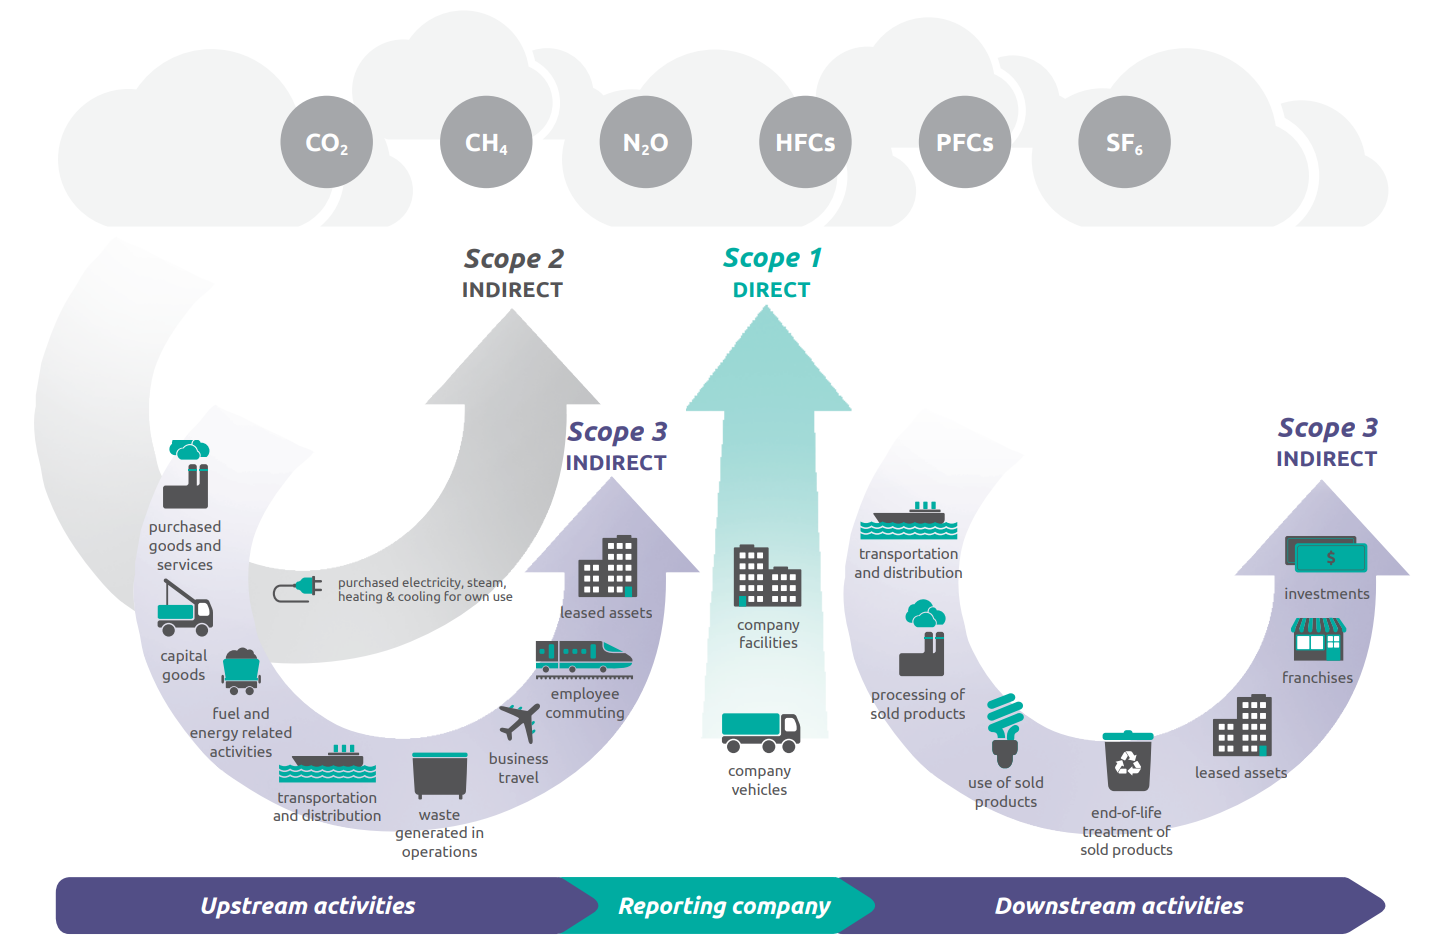
\includegraphics[width=0.8\textwidth]{figures/chapter2_figures/ghg_scope.png}
\end{figure}

In their most complete form, border carbon adjustments cover all goods that cross the border, not just imports. Just like highly-regulated domestic production will likely have a cost disadvantage in the domestic market, highly-regulated exports will likely have a cost disadvantage in foreign markets. To prevent jurisdictions with ambitious climate policy from losing their exports requires some way to adjust the price of exports. This is the purpose of an \emph{export rebate}, often just called an \emph{output rebate}.

An output rebate pays back a flat rate to domestic producers for every unit they export. While carbon taxes on imports try to even the playing field between highly regulated and less regulated producers in domestic markets, output rebates try to even the playing field between highly regulated and less regulated producers on foreign markets. For instance, if US fertilizer manufacturers export much of their product, imposing a domestic carbon tax raises these manufacturers’ costs relative to their competitors overseas. This cost differential may allow foreign fertilizer manufacturers to retake some of the (foreign) market share from US fertilizer manufacturers. This increased foreign production will lead to greater GHG emissions associated with the foreign fertilizer market, a problem that may be exacerbated if foreign manufacturers were already more emissions intensive than US manufacturers.

Output rebates lack the same intuitive appeal that an emissions tax on imports have. After all, why should we tax manufacturers only to pay them back? Why not just tax manufacturers the difference between the original emissions tax and the output rebate? The first reason is a matter of accounting. Output rebates only apply to exports, so reducing the tax on all goods would not differentiate between the goods that should and should not receive a subsidy to avoid leakage. The second reason is a matter of incentives. Output rebates are not refunds on emissions taxes, as the government pays these out for every unit of output rather than for every ton of GHG emissions. In a world where goods had a fixed emissions intensity, this difference would not matter. Thankfully though, there are ways to reduce emissions without reducing output (e.g., switching to cleaner inputs or installing smokestack scrubbers). Thus, an output rebate will maintain the same abatement incentive on exports, while also allowing domestic producers to maintain their ability to compete in foreign markets. The low volume of US manufacturing exports relative to imports means that these are not typically the primary concern in anti-leakage policy.

%\begin{figure}
%\caption{Leakage with an Emissions Tax on Imports}
%\centering
%\singlespacing
%\footnotesize
%\begin{tikzpicture}[scale = 0.5]
%	\draw[very thick, <->] (0, 11) node[left]{$p$} -- (0, 0) -- (11, 0) node[below, text width = 2cm]{Domestic Quantity};
%	\draw[very thick, <->] (15, 11) node[left]{$p$} -- (15,0) -- (26, 0) node[below, text width = 2cm]{Imported Quantity};
%	\fill[orange!80!, opacity = 0.6] (3.5, 3.75) -- (3.5, 1.75) -- (4.5, 2.25) -- (4.5, 4.25) -- cycle;
%	\fill[yellow!80!, opacity = 0.6] (4.5, 2.25) -- (5.5, 2.75) -- (5.5, 4.75) -- (4.5, 4.25) -- cycle;
%	\fill[orange!80!, opacity = 0.6] (16.75, 4.75) -- (16.75, 2.75) -- (17.75, 3.75) -- (17.75, 5.75) -- cycle;
%	\fill[yellow!80!, opacity = 0.6] (16.25, 4.25) -- (16.25, 2.25) -- (16.75, 2.75) -- (16.75, 4.75) -- cycle;
%	\fill[orange!80!, opacity = 0.6] (21.25, 9.25) -- (21.25, 7.25) -- (22.25, 8.25) -- (22.25, 10.25) -- cycle;
%	\fill[yellow!80!, opacity = 0.6] (20.75, 8.75) -- (20.75, 6.75) -- (21.25, 7.25) -- (21.25, 9.25) -- cycle;
%	\draw[very thick, EAPblue] (0,0) -- (10, 5) node[right]{MC$_d$};
%	\draw[very thick, EAPgreen] (0,2) -- (10, 7) node[right]{MC$_d$ $+$ Tax};
%	\draw[very thick, gray] (0, 10) -- (10,0) node[pos=.2, above right,text width = 1.5cm]{Domestic Demand}; 
%	\draw[very thick, EAPred] (0,5.5) -- (9, 1) -- (10, 0) node[pos=.8, above right, text width = 1.5cm]{Residual Demand};
%	\draw[very thick, EAPred] (0, 6.5) -- (7,3) -- (10, 0);
%	\draw[very thick, gray] (15, 10) -- (25, 0) node[pos=.8, above right,text width = 1.5cm]{Domestic Demand}; 
%	\draw[very thick, EAPblue] (15, 1) -- (24, 10) node[right, text width = 1.5cm]{MC$_f$};
%	\draw[dashed, thick] (5.5, 4.75) -- (5.5, 0) node[below]{$q_d$};
%	\draw[dashed, thick] (3.5, 3.75) -- (3.5, 0) node[below]{$q_d'$};
%	\draw[dashed, thick] (4.5, 4.25) -- (4.5, 0) node[below]{$q_d''$};
%	\draw[dashed, thick] (0, 3.75) node[left]{$p'$} -- (21.25, 3.75);
%	\draw[dashed, thick] (0, 2.75) node[left]{$p$} -- (22.25, 2.75);
%	\draw[dashed, thick] (0,4.25) node[left]{$p''$} -- (20.75, 4.25);
%	\draw[dashed, thick] (16.75,4.75) -- (16.75, 0) node[below, yshift = -3pt, xshift = 2pt]{$q_f$};
%	\draw[dashed, thick] (17.75, 5.75) -- (17.75, 0) node[below]{$q_f'$};
%	\draw[dashed, thick] (16.25, 4.25) -- (16.25, 0) node[below]{$q_f''$};
%	\draw[dashed, thick] (22.25, 10.25) -- (22.25, 0) node[below]{$q$};
%	\draw[dashed, thick] (21.25, 9.25) -- (21.25, 0) node[below]{$q'$};
%	\draw[dashed, thick] (20.75, 8.75) -- (20.75, 0) node[below]{$q''$};
%	\draw[EAPred, very thick] (15, 3) -- (23, 11) node[right]{MC$_f$ $+$ Tax};
%	%\draw[thick, <-] (5, 4) -- (8, 8) node[above, text width = 2cm, align=center]{Domestic Abatement};
%	%\draw[thick, <-] (16.7, 4.5) -- (18, 8) node[above, text width = 2cm, align=center]{Emissions Leakage}; 
% 	%\draw[thick, <-] (21.6, 8) -- (23, 6) node[below right, text width = 1.6cm, align=center]{Net Abatement};
% 	\node at (5.5, 12) {Domestic Market};
% 	\node at (20.5, 12) {Foreign Imports}; 
%\end{tikzpicture}
%\end{figure}


\subsection{Distributional Considerations in Market-Based Policy Design}

\textit{Forthcoming}.


%%%%%%%%%%%